\documentclass[a4paper]{report}

% Utilisation des différents paquets :
\usepackage[french]{babel}
\usepackage[T1]{fontenc}
\usepackage{hyperref}
\usepackage{hhline}
\usepackage{multirow}
\usepackage{fancyhdr}
\usepackage{lastpage}
\usepackage{graphicx}
\usepackage{mathtools, bm}
\usepackage{amssymb, bm}
\usepackage{amsmath}
\usepackage{listings}
\usepackage{geometry} 
\usepackage{caption}
\usepackage{xcolor}
\usepackage[most]{tcolorbox}
\usepackage{inconsolata}
\usepackage{amsfonts}
\usepackage{algorithm}
\usepackage{algorithmic}
\usepackage{stmaryrd}

% Informations sur le document :
\title{D�veloppement web : Kunu }
\author{\sc{CROCE Baptiste, JACQUELIN Anthony, MARZOOK Cyril}}
\date{\emph{Vendredi 14 juin 2019}}

% Personnalisation de la numérotation des sections et sous-sections
\renewcommand\thesection {\Roman{section}}

\setcounter{section}{0}


% Quelques constantes : 
\makeatletter
  \let\thetitle\@title
  \let\theauthor\@author
  \let\thedate\@date
\makeatother



% Personnalisation des en-têtes et pieds de page :
\pagestyle{fancy}
\fancyhead[L]{\fontsize{13}{22} \selectfont \thetitle}
\fancyhead[R]{
\includegraphics[scale=0.04]{logo.png}}
\fancyhead[C]{}
    \renewcommand{\footrulewidth}{0.4pt}
\fancyfoot[L]{\rightmark}
\fancyfoot[R]{\thepage /\pageref{LastPage}}
\fancyfoot[C]{}



\newtcblisting[auto counter]{sexylisting}[2][]{sharp corners, 
    fonttitle=\bfseries, colframe=gray, listing only, 
    listing options={basicstyle=\ttfamily,language=java}, 
    title=Listing \thetcbcounter: #2, #1}


% Début du document
\begin{document}
    \maketitle
      \tableofcontents
        \newpage
	\
	\
	\
	\
	\
 \section{Introduction}
 
 	Au cours de ce projet, nous avons d� mettre en place un site complet nomm� Kunu.
	\\
				//Photo bienvenue sur Kunu�//
				\\
Le principe de ce site? R�unir tout ce qui peux �tre important/int�ressant a savoir lorsque l'on s'int�resse au naturisme. Et ce, autant pour la partie int�raction entre adepte de ce choix de vie, qu?information sur le sujet ou cr�ation/r�servation de s�jours. Afin de mener � bien ce projet, nous nous sommes grandement int�ress� aux cahiers des charges fournit, mais plus pr�cis�ment aux annexes, ainsi qu'au site d�j� existant. Car pour retranscrire un site, qui refl�te correctement ce que l'on veux, il faut d'abord comprendre les enjeux et la vision du demandeur. Ainsi nous avons d�cid� de r�aliser un site assez �pur� ou la majorit� des fonctionnalit�s se trouvent sur la page d'accueil, accessible depuis un bandeau de haut de page. 
Pour r�aliser tout cela, nous avons donc utiliser plusieurs technologies, sur lesquelles on reviendra au moment ou parle de leurs utilisations, parmi elle on peux compter html, css, js, php, dom, ajax et mysql.
 \newpage
	\
	\
	\
	\
	\
	\
\section{Pr�sentation du projet}
 \newpage
	\
	\
	\
	\
	\
	\


\section{Choix technologiques}
 \newpage
	\
	\
	\
	\
	\
	\

\section{Choix de design}
 \newpage
	\
	\
	\
	\
	\
	\
\section{Descriptions des pages}
\subsection{Accueil}
\\
\begin{center}
 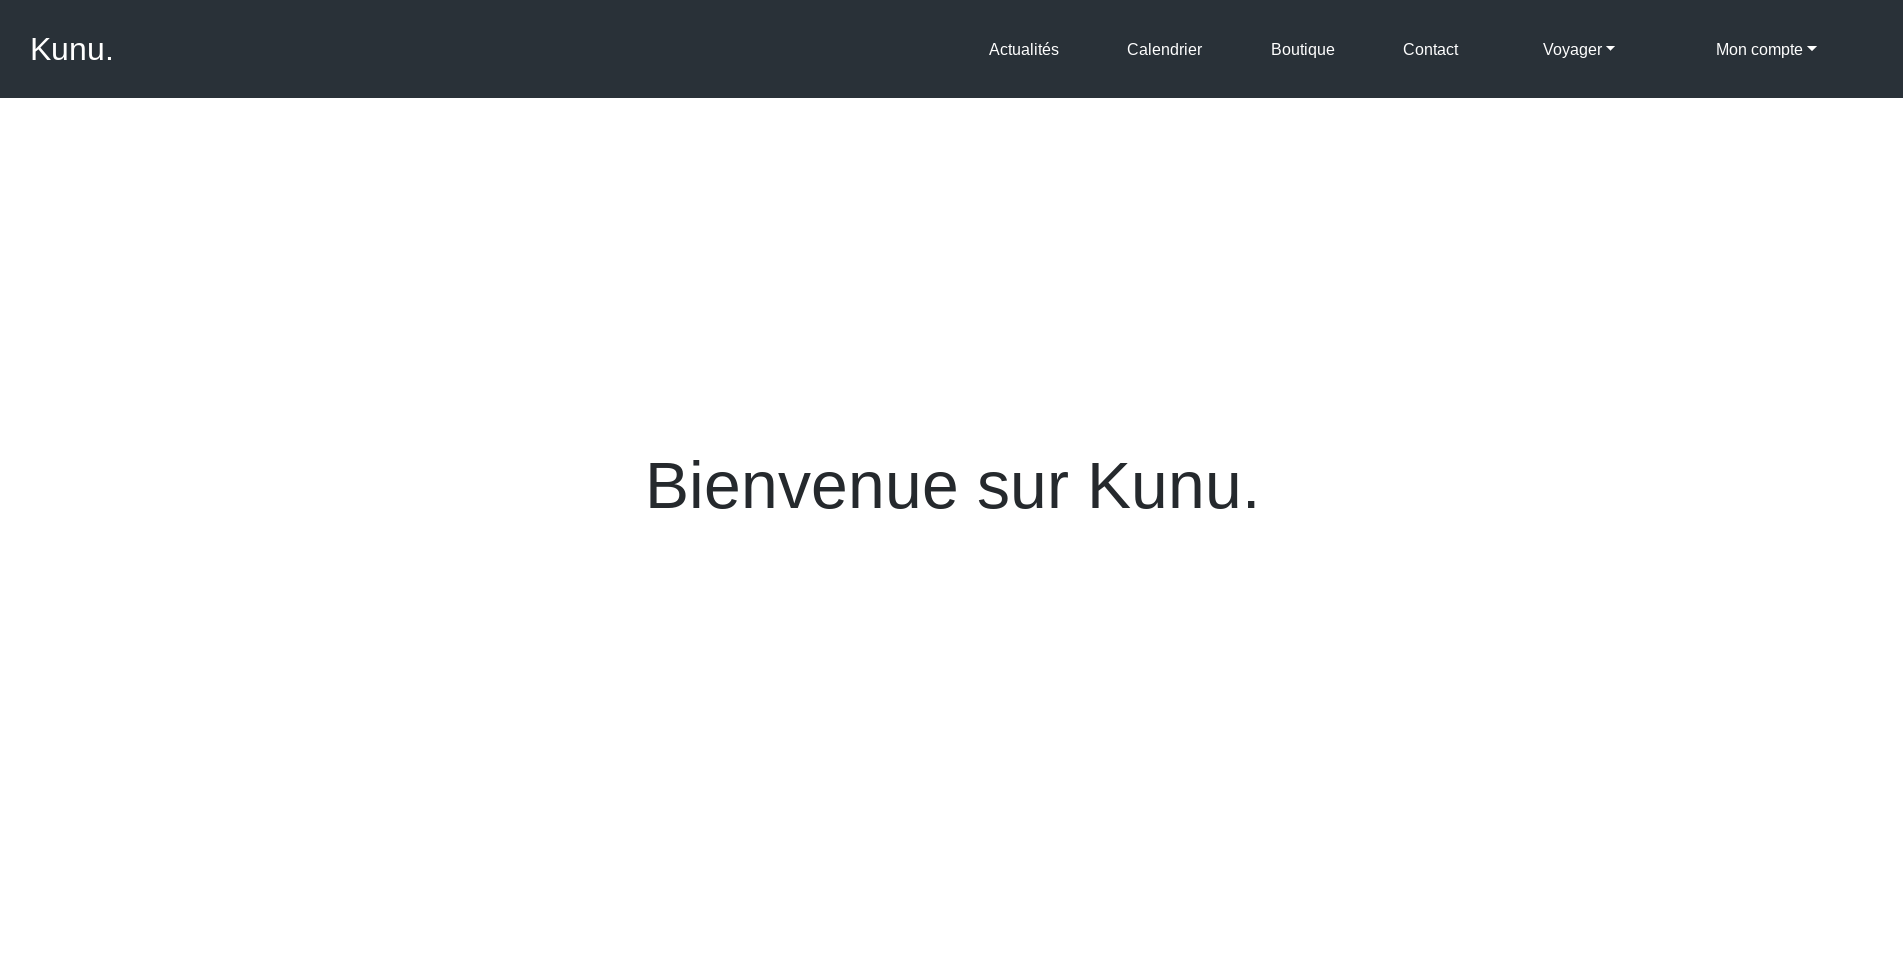
\includegraphics[scale=0.4]{img/Accueil.png}
\end{center}
\\
\\
\begin{center}
 
\includegraphics[scale=0.4]{img/AccueilTel.png}
\end{center}
\\
 \newpage
	\
	\
	\
	\
	\
	\

\subsection{Actualit�s}
\\
\begin{center}
 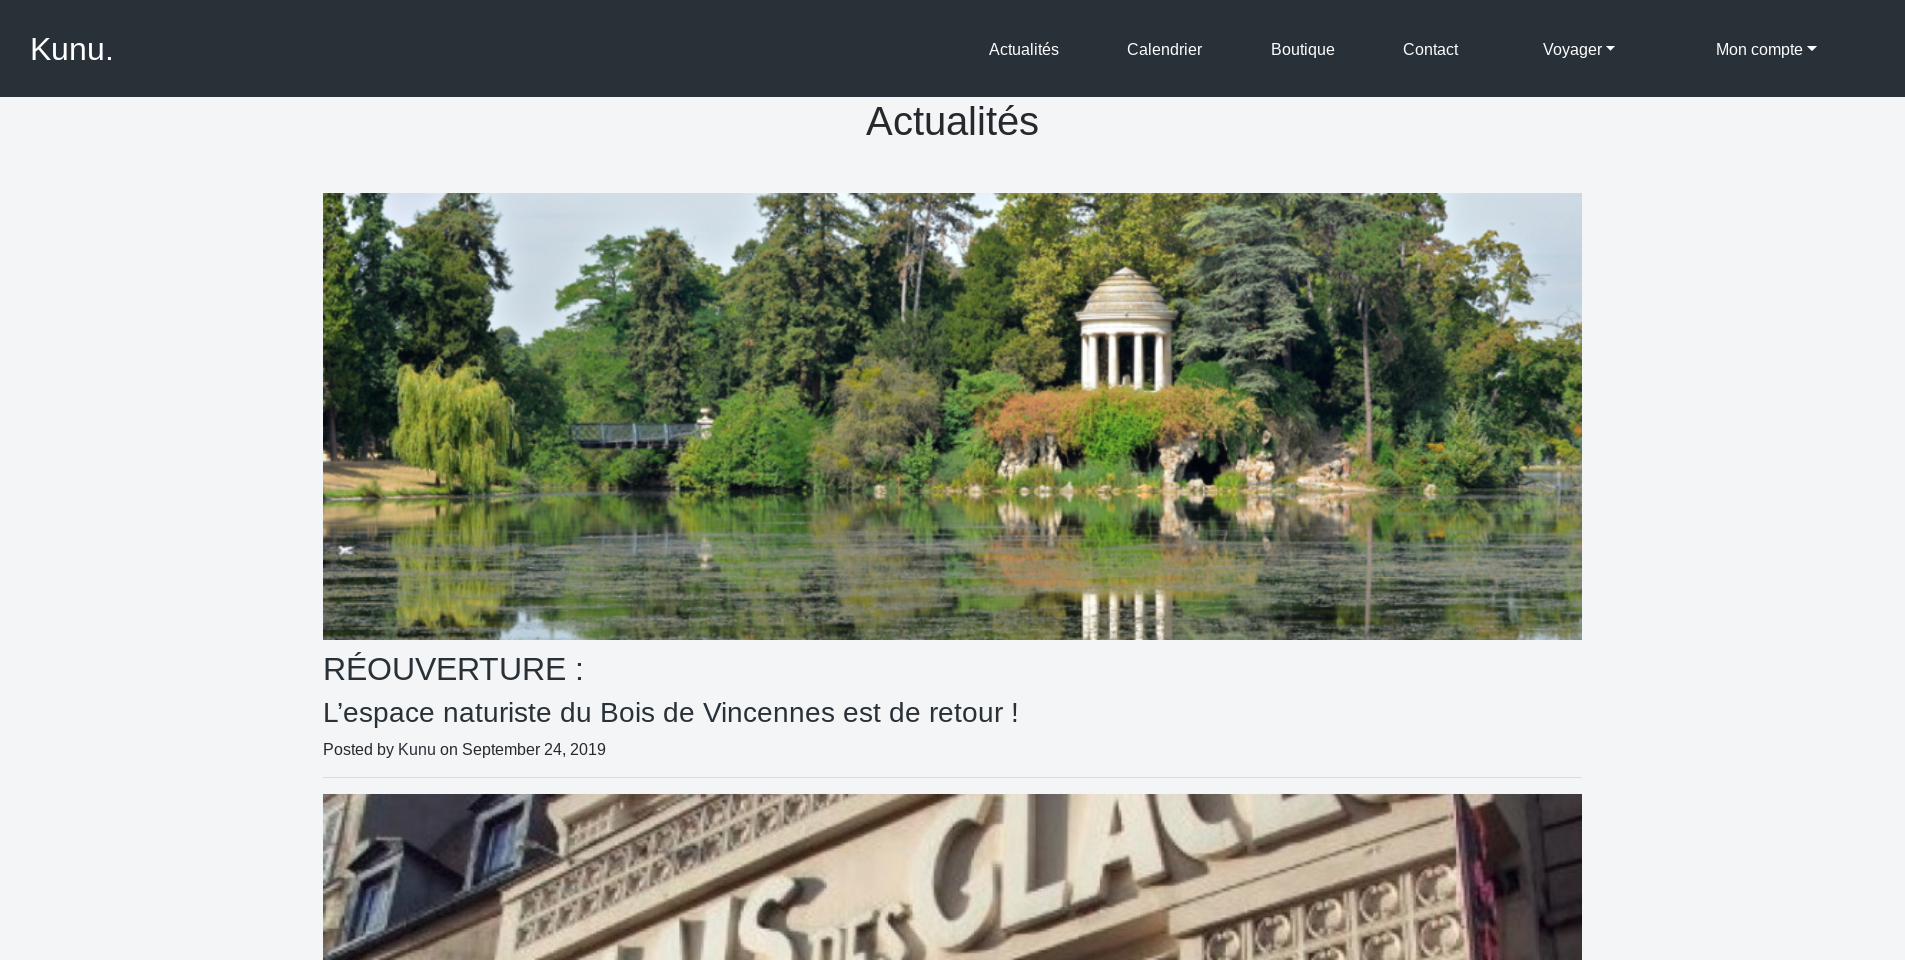
\includegraphics[scale=0.4]{img/Actualite.png}
\end{center}
\\

 \newpage
	\
	\
	\
	\
	\
	\

\subsection{Calendrier}
\\
\begin{center}
 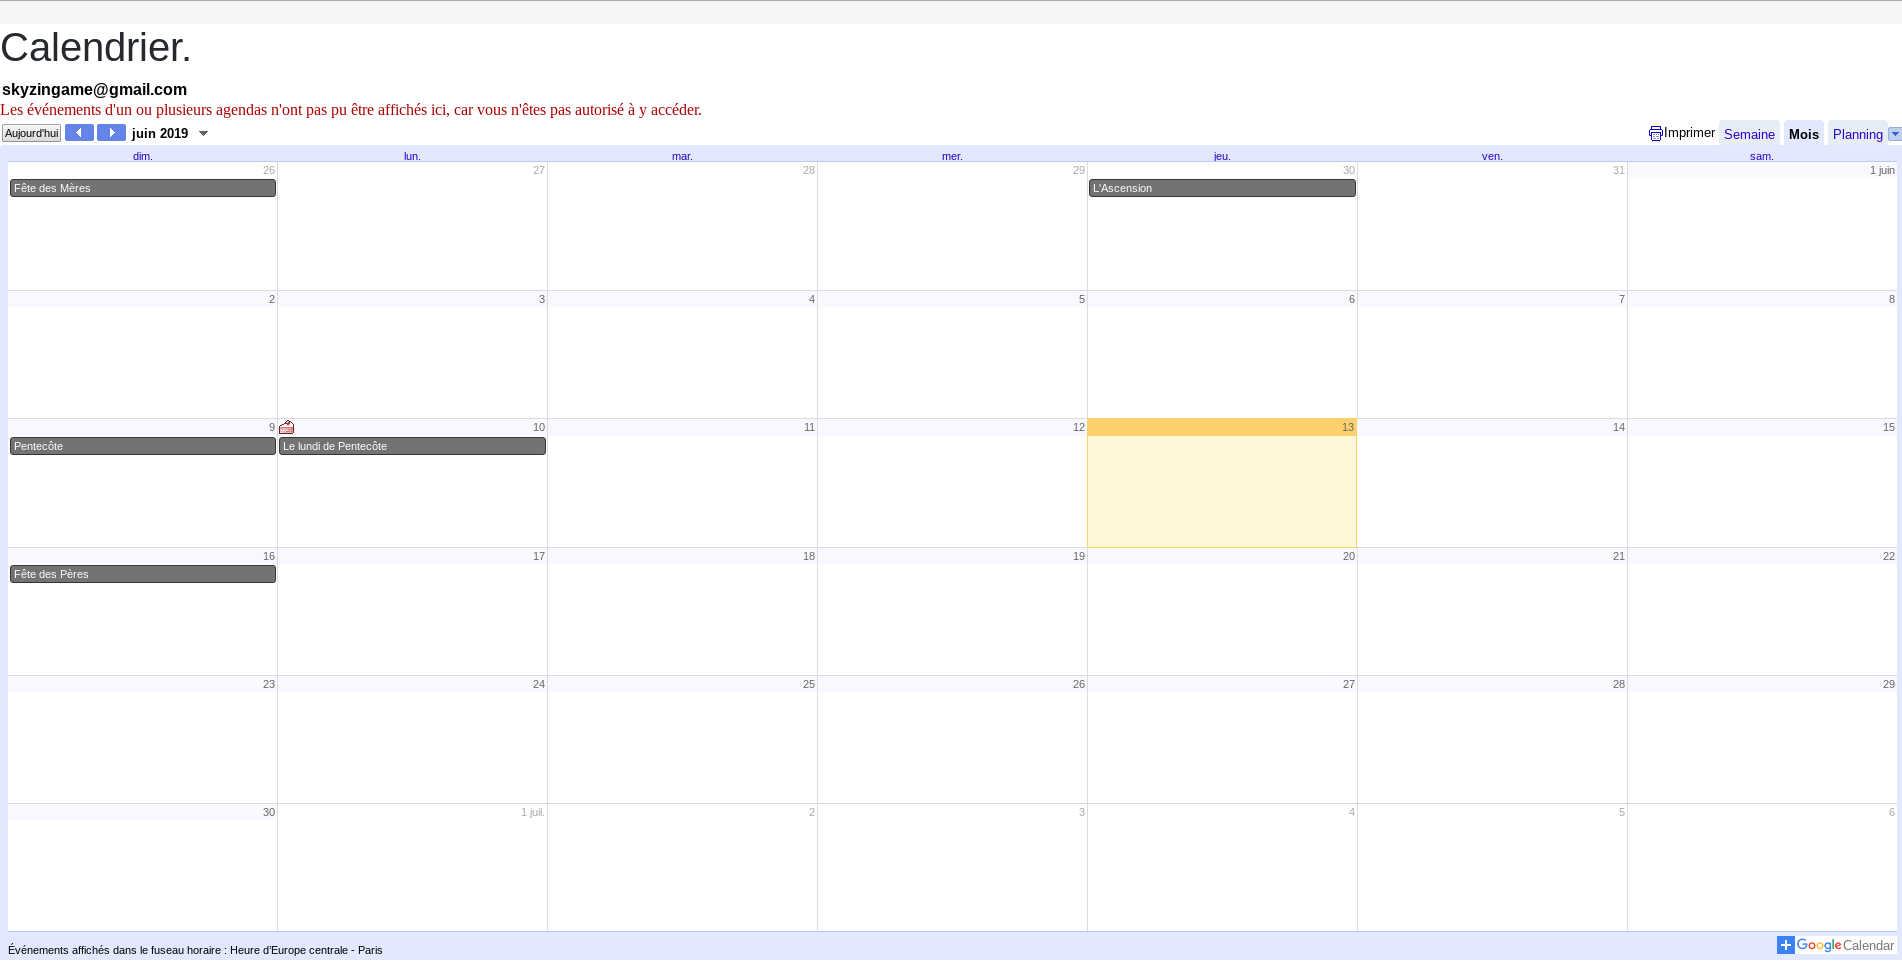
\includegraphics[scale=0.4]{img/Calendrier.png}
\end{center}
\\

 \newpage
	\
	\
	\
	\
	\
	\
	
\subsection{Boutique}
\\
\begin{center}
 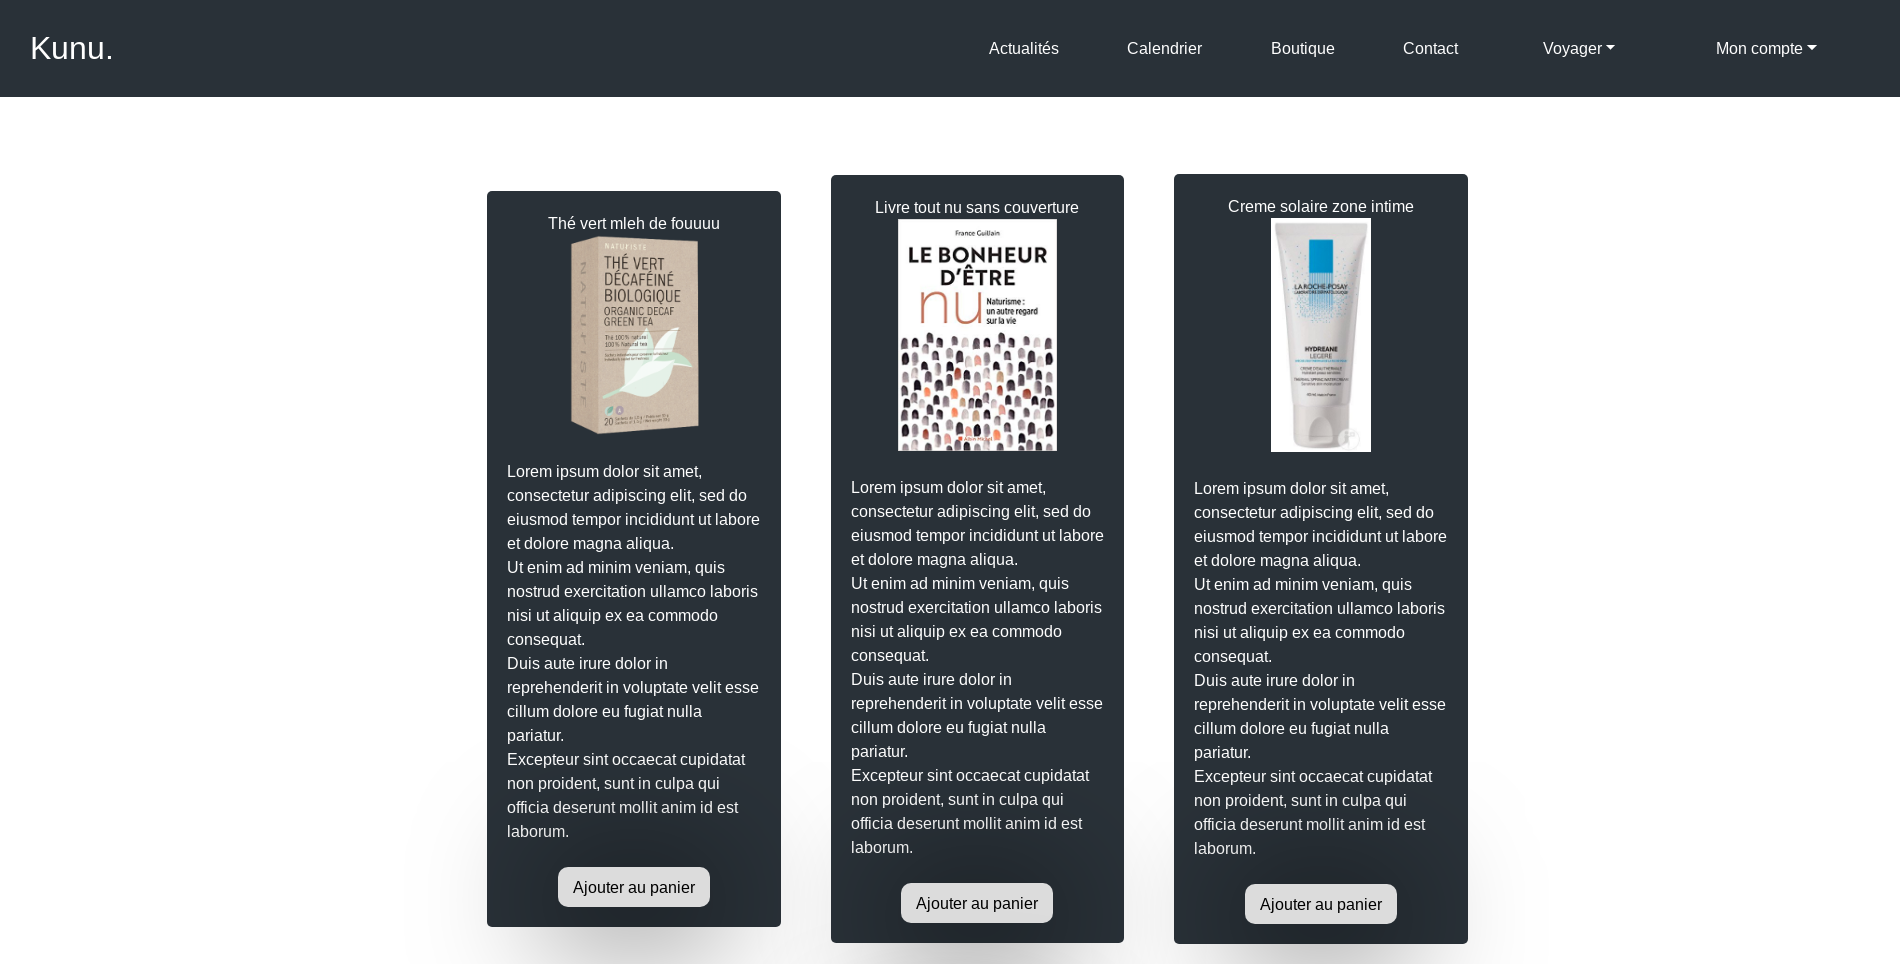
\includegraphics[scale=0.4]{img/Boutique.png}
\end{center}
\\

 \newpage
	\
	\
	\
	\
	\
	\
	
\subsection{Panier}
\\
\begin{center}
 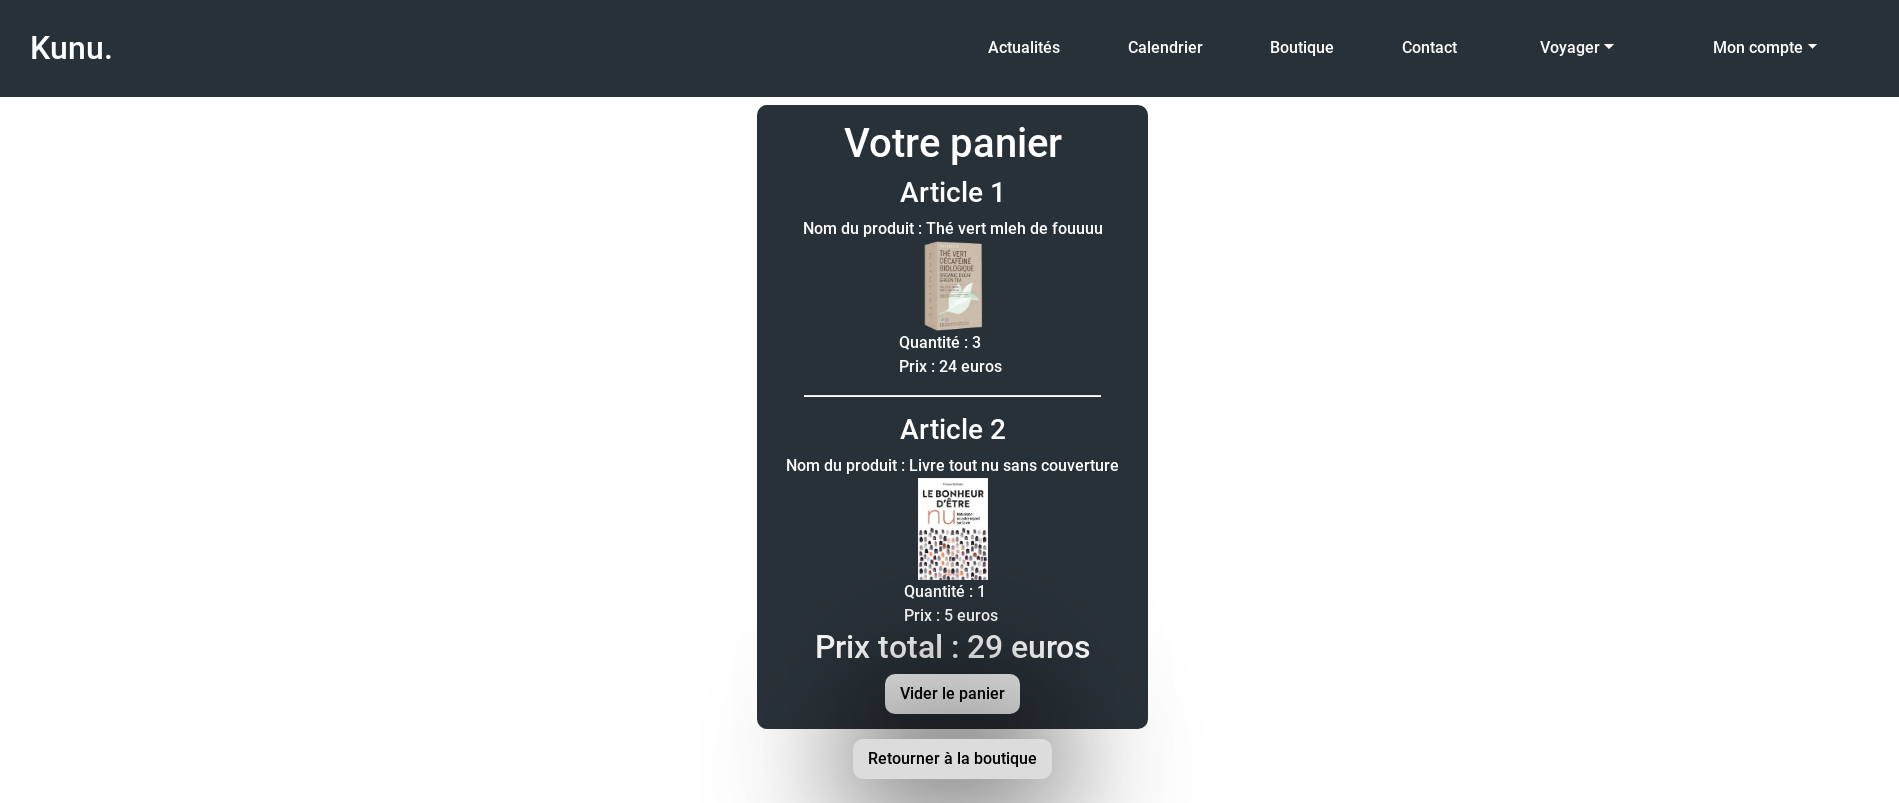
\includegraphics[scale=0.4]{img/Panier.png}
\end{center}
\\

 \newpage
	\
	\
	\
	\
	\
	\
	

\subsection{Contact}
\\
\begin{center}
 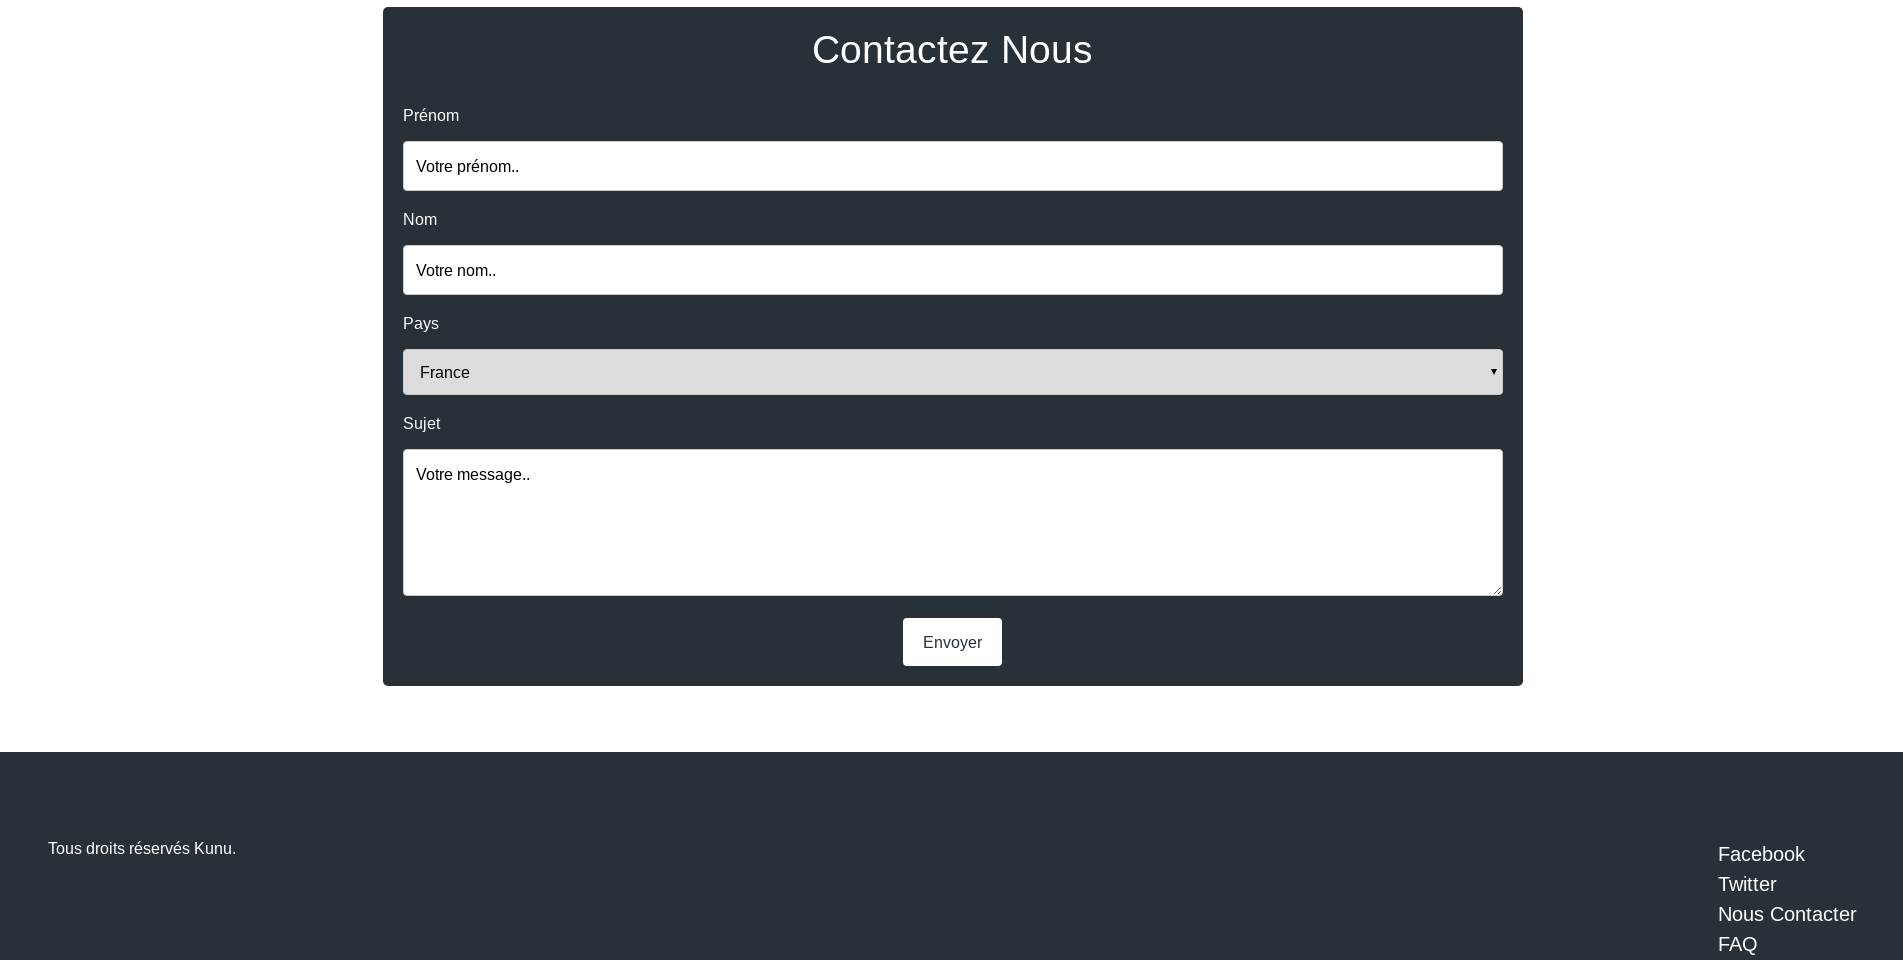
\includegraphics[scale=0.4]{img/Contact.png}
\end{center}
\\

 \newpage
	\
	\
	\
	\
	\
	\
	
\subsection{Voyager}
\\
\begin{center}
 
\includegraphics[scale=0.4]{img/Voyager.png}
\end{center}
\\

\subsubsection{Cr�er un s�jour}
\\
\begin{center}
 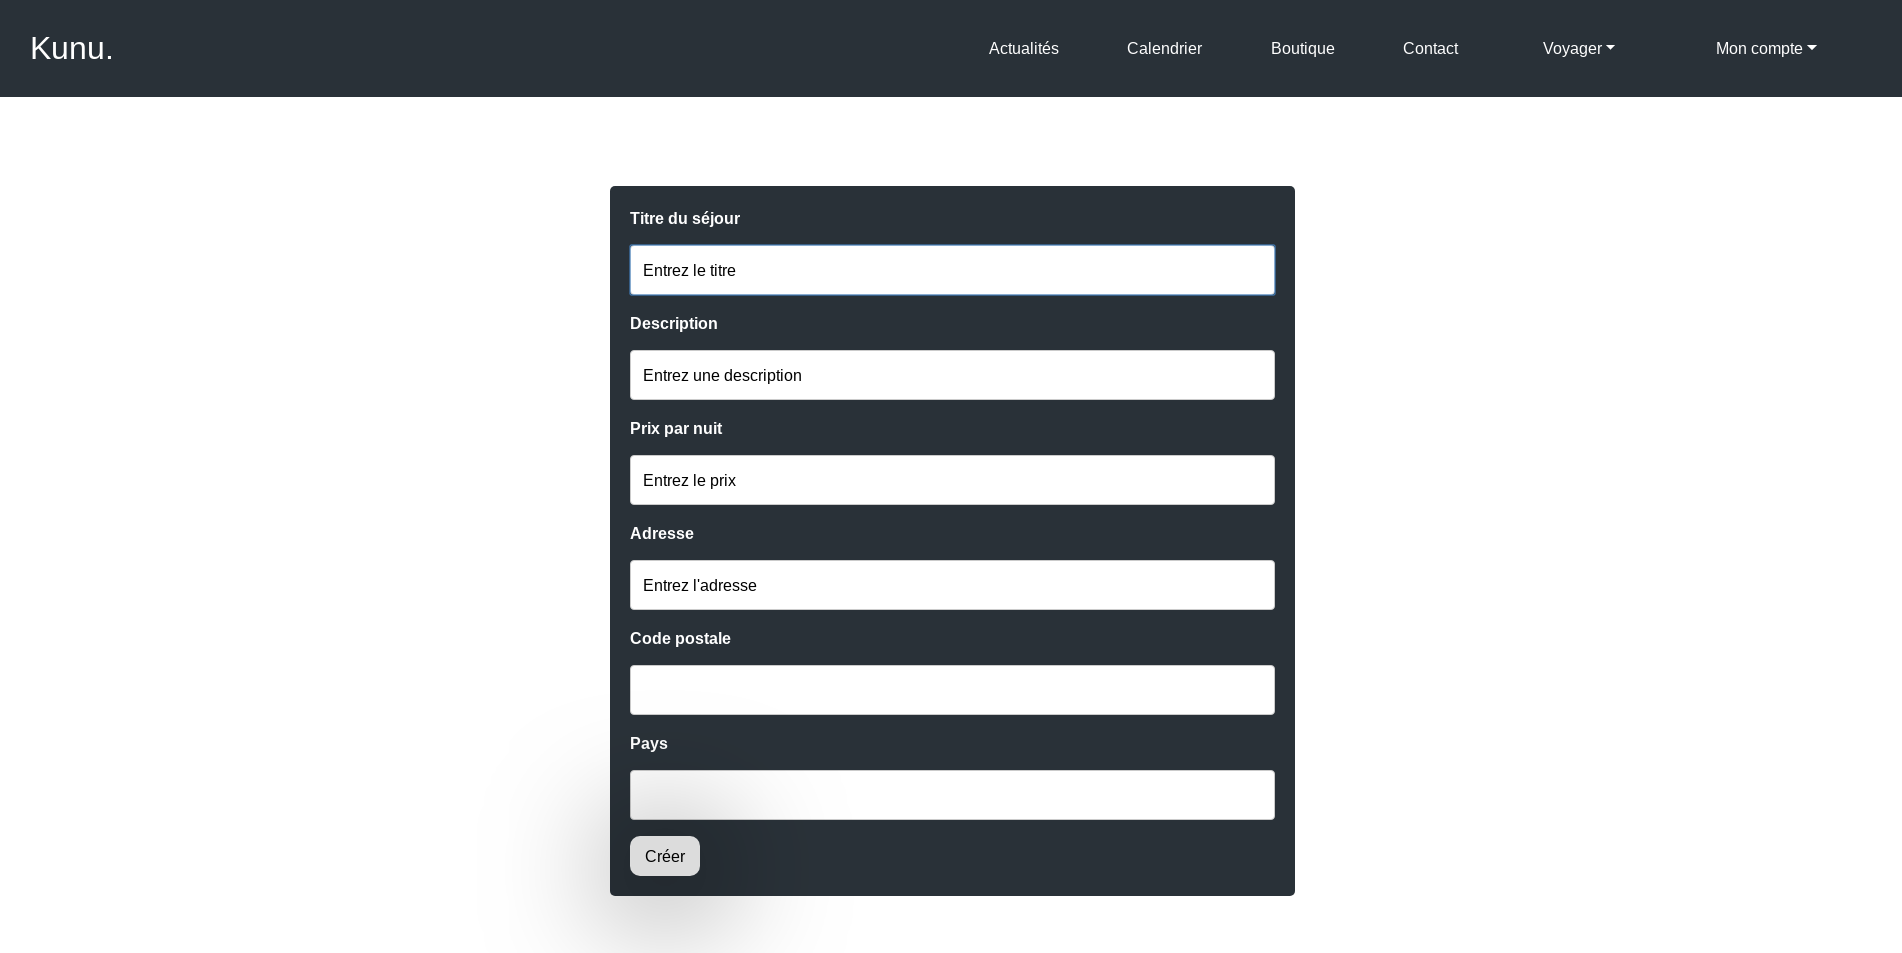
\includegraphics[scale=0.4]{img/CreerSejour.png}
\end{center}
\\

\subsubsection{R�server un s�jour}
\\
\begin{center}
 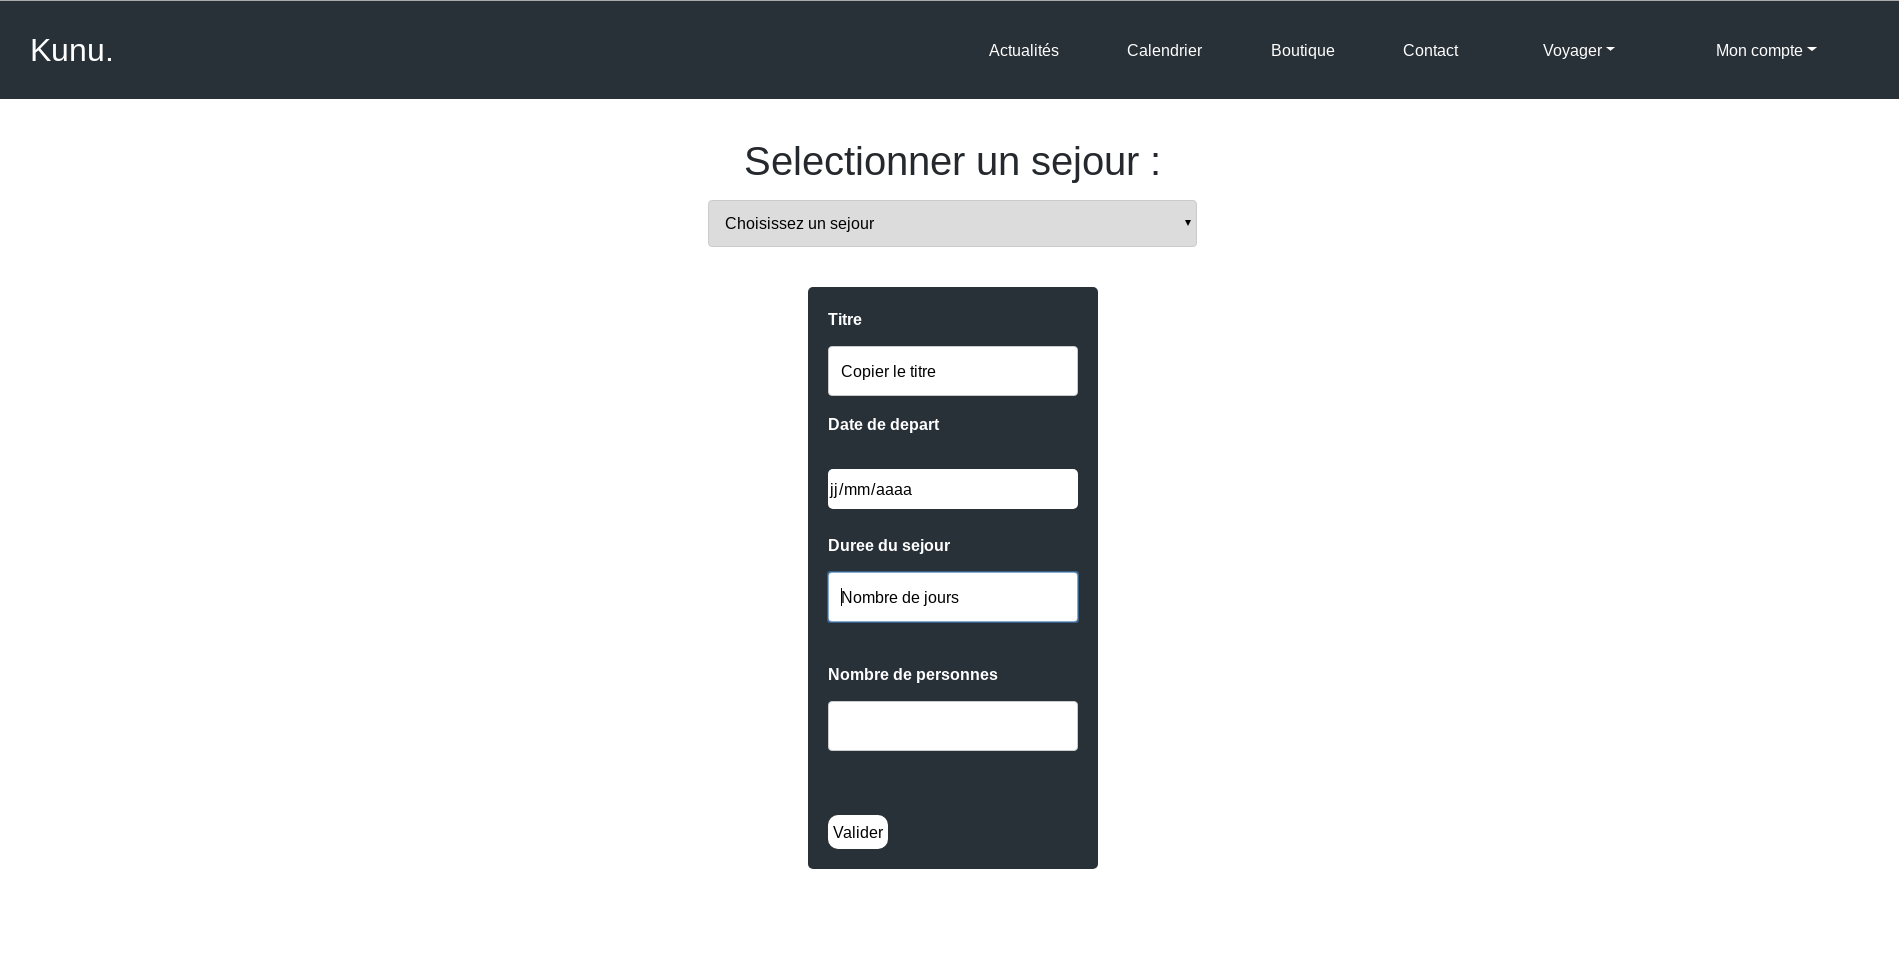
\includegraphics[scale=0.4]{img/Sejour1.png}
\end{center}
\\
\\
\begin{center}
 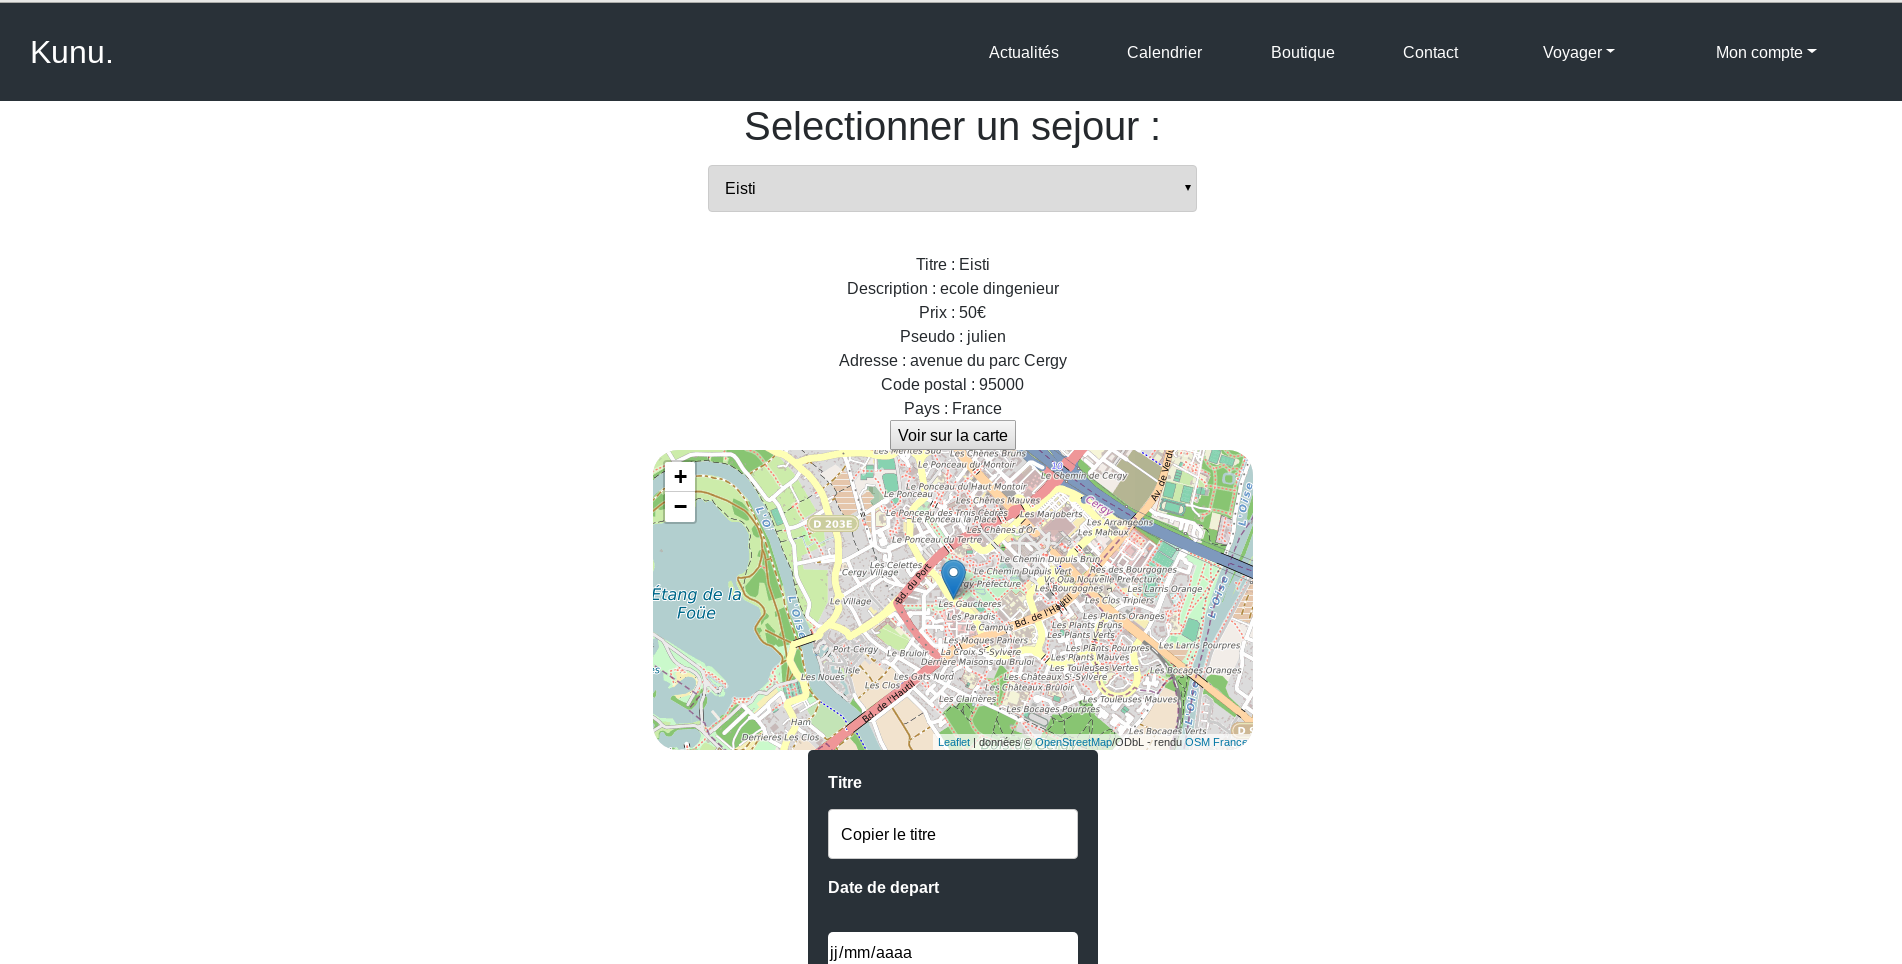
\includegraphics[scale=0.4]{img/Sejour2.png}
\end{center}
\\
 \newpage
	\
	\
	\
	\
	\
	\
	
\subsection{Mon compte}
\\
\begin{center}
 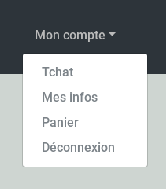
\includegraphics[scale=0.4]{img/Compte.png}
\end{center}
\\

\subsubsection{Mes infos}
\\
\begin{center}
 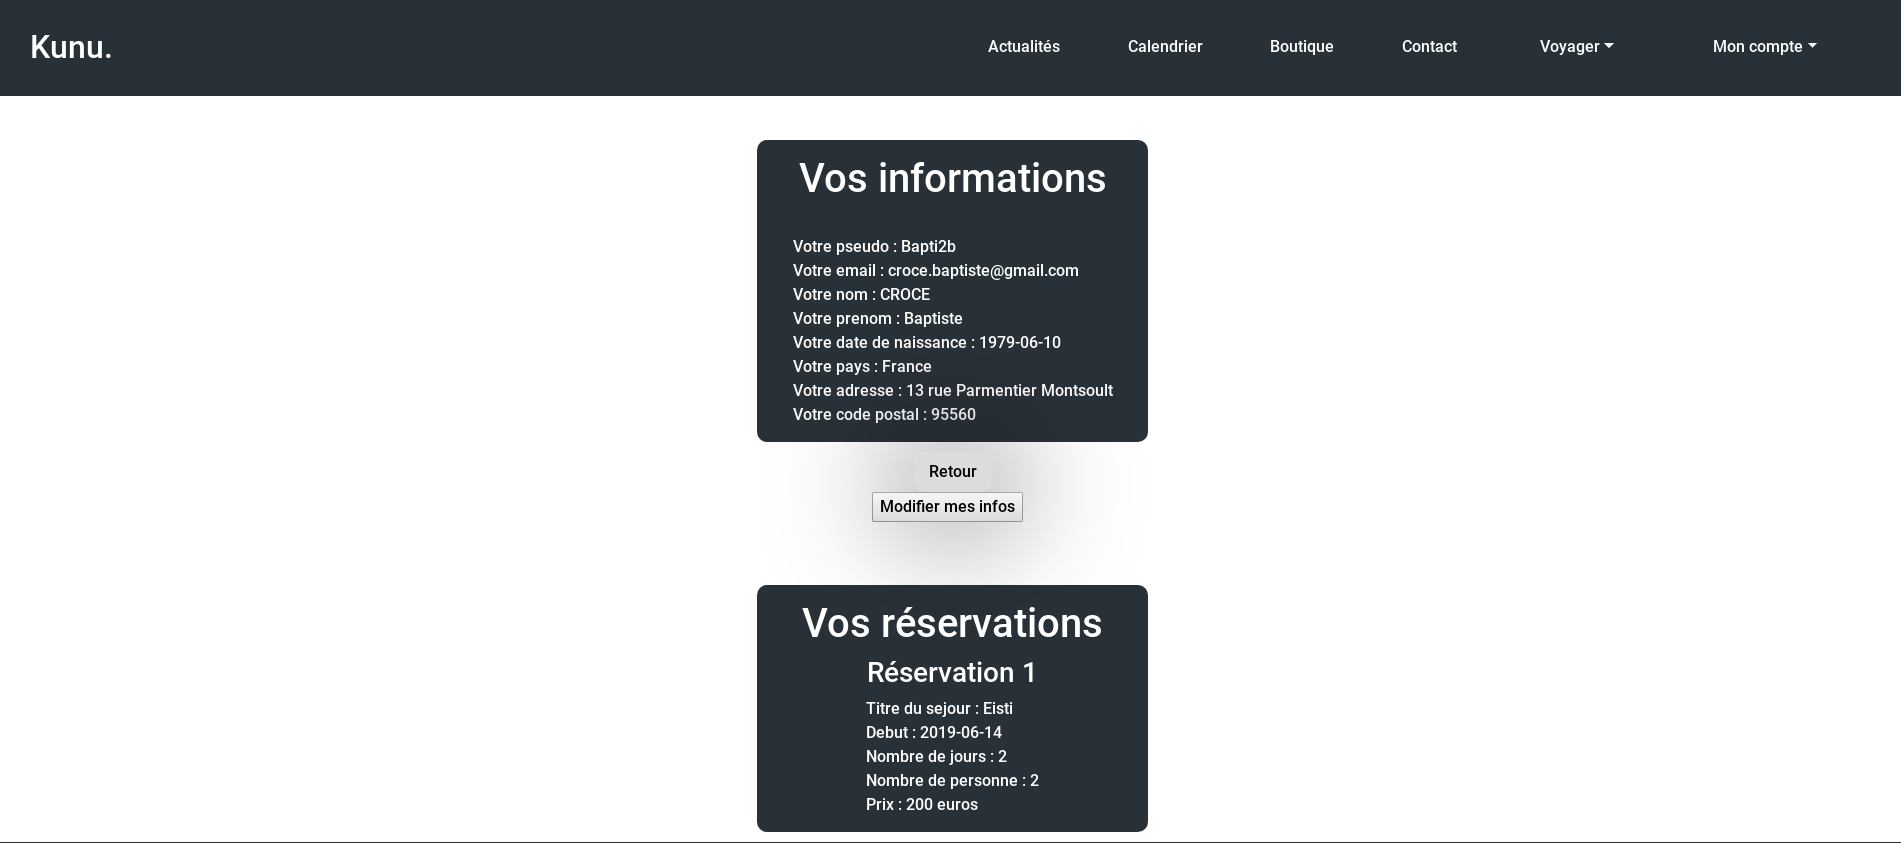
\includegraphics[scale=0.4]{img/Infos.png}
\end{center}
\\

\subsubsection{Deconnexion}
\\
\begin{center}
 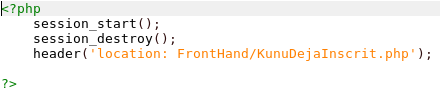
\includegraphics[scale=0.4]{img/Deconnexion.png}
\end{center}
\\

 \newpage
	\
	\
	\
	\
	\
	\
	
\subsection{Tchat}
\\
\begin{center}
 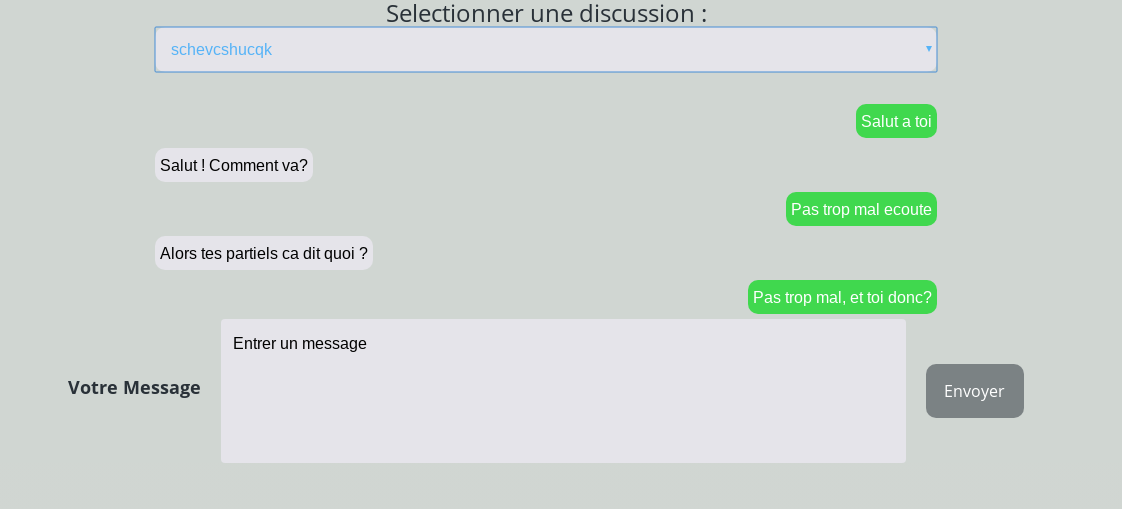
\includegraphics[scale=0.4]{img/Tchat.png}
\end{center}
\\




 \newpage
	\
	\
	\
	\
	\
	\
\section{R�partitions des t�ches}
 \newpage
	\
	\
	\
	\
	\
	\
\section{Bilan et perspectives}


 \end{document}
